% !TEX encoding = UTF-8
% !TEX TS-program = pdflatex
% !TEX root = ../tesi.tex

\chapter{Analisi del contesto aziendale}
\label{cap:contesto-aziendale}

\section{L'azienda Sync Lab}
Sync Lab nasce come \emph{software house} nel 2002, per poi crescere rapidamente nel mercato del \gls{ICT}. In seguito ad una maturazione delle competenze tecnologiche, metodologiche ed applicative nel dominio del \emph{software}, si è tramutata in \gls{System Integrator} conquistando significative fette di mercato nei settori: \emph{mobile}, videosorveglianza e sicurezza delle infrastrutture informatiche aziendali. Attualmente vanta più di 150 clienti diretti e finali, 200 dipendenti e 5 sedi distribuite in tutta Italia. 

\begin{figure}[!h]
  \centering
  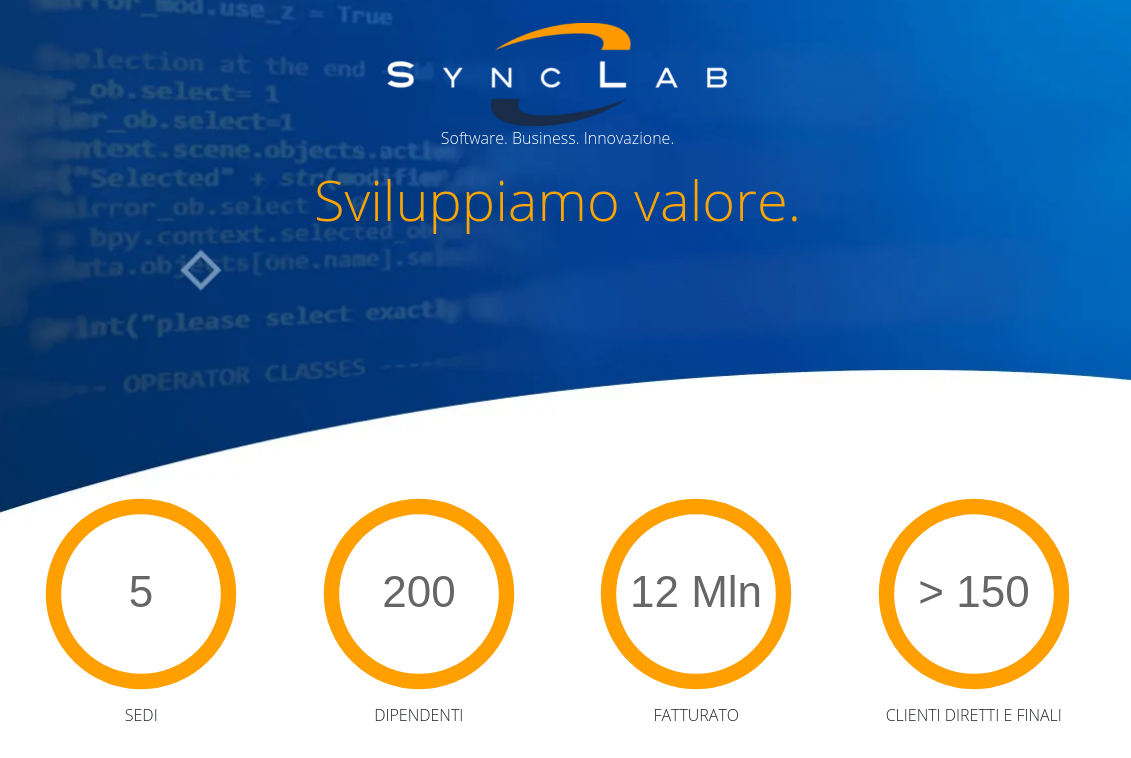
\includegraphics[width=\textwidth]{capitolo1/motto-synclab.png}
  \caption{Motto di Sync Lab e le sue statistiche}
  \textbf{Fonte}: \href{https://www.synclab.it}{https://www.synclab.it}
\end{figure}

Sync Lab consegue l'obiettivo principale di supportate il cliente nella realizzazione, messa in opera e controllo di soluzioni IT, sia dal punto di vista tecnologico, sia nel governo del cambiamento organizzativo. Nel corso degli anni ha aumentato la propria qualità organizzativa e produttiva, riuscendo ad acquisire le seguenti 4 certificazioni: ISO 9001, ISO 14001, ISO 27001 e ISO 45001.

\section{Prodotti}
Sync Lab è un'azienda di consulenza tecnologica che mette a disposizione ai suoi clienti competenze altamente qualificate ed esperienza nel dominio tecnologico. Grazie a questo, le aziende possono affrontare i cambiamenti tecnologici e di mercato rimanendo sempre competitive nell'attuale contesto di trasformazione digitale. L'azienda opera principalmente nel settore informatico e, più precisamente, nel \emph{business consultancy}, \emph{IT consultancy} e \emph{project financing}.

\begin{figure}[!h]
  \centering
  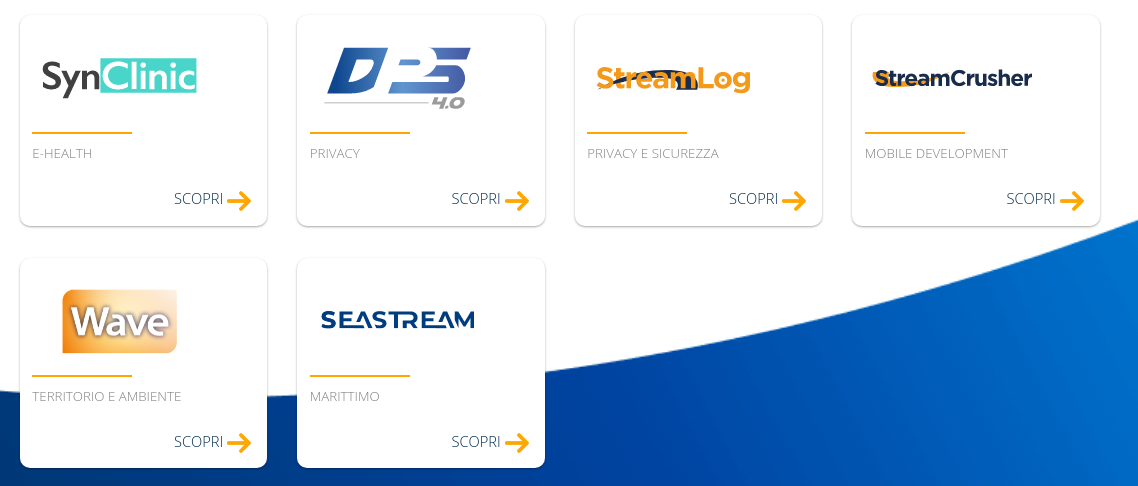
\includegraphics[width=\textwidth]{capitolo1/prodotti-synclab.png}
  \caption{I prodotti di Sync Lab}
  \textbf{Fonte}: \href{https://www.synclab.it/prodotti.php}{https://www.synclab.it/prodotti.php}
\end{figure}

In questo ambito, Sync Lab, vanta numerosi prodotti:
\begin{itemize}
  \item \textbf{SynClinic}: \emph{software} che facilita la gestione di una struttura sanitaria. Utilizzabile in \emph{cloud} e \gls{on premises}, gestisce, organizza e monitora tutte le fasi del percorso di cura del paziente, integrandosi perfettamente con i servizi regionali: fascicolo sanitario elettronico, ricetta dematerializzata e CUP regionale;
  
  \item \textbf{DPS 4.0}: consiste in una soluzione web per la gestione del GDPR, con una piattaforma guidata per aggiornare e modificare automaticamente i documenti di privacy in modo conforme agli standard di riferimento europei;
  
  \item \textbf{StreamLog}: rappresenta un sistema finalizzato al soddisfacimento dei requisiti fissati al garante, ovvero effettua il controllo degli accessi ai sistemi in modo semplice e veloce. La piattaforma è basata su \emph{framework open source} allo stato dell'arte e, in particolare, su un'innovativa tecnologia di \emph{streaming}, frutto del laboratorio di ricerca e sviluppo Sync Lab;
  
  \item \textbf{StreamCrusher}: soluzione \emph{software} che è in grado di raccogliere, indicizzare, ed interpretare la grande mole di dati che giornalmente genera qualsiasi azienda. In seguito, produrrà un resoconto con tutte le informazioni utili al centro informatico, per identificare criticità o eventuali opportunità di \emph{business};
  
  \item \textbf{Wave}: nato dal laboratorio di ricerca e sviluppo, è un \emph{plugin} della piattaforma \emph{Milestone System A/S} che permette di avere una visione geografica della distribuzione delle telecamere installate nel territorio e di capire la copertura garantita da un'installazione reale;
  
  \item \textbf{SeaStream}: piattaforma che migliora l'efficienza, la sicurezza e il processo di innovazione del settore marittimo, mettendo a disposizione strumenti per il monitoraggio e tracciamento delle navi e per la gestione portuale.  
\end{itemize}

\section{Tipologia di clientela}
La clientela che si affida a Sync Lab è molto vasta, comprendendo al suo interno aziende pubbliche e private, piccole e grandi imprese. Tutte le aziende elencate in precedenza si mettono in contatto con Sync Lab per migliorare i propri processi interni, andando così ad incrementare la propria efficienza sotto l'aspetto lavorativo. Riuscendo a soddisfare qualsiasi richiesta, Sync Lab può vantare clienti come: la regione Lazio, Trenitalia, il ministero dell'economia e delle finanze, Rai, Unicredit, Vodafone e Intesa San Paolo. Per ogni settore, l'azienda è in continua ricerca di nuove opportunità e soluzioni cercando di allargare sempre più il proprio campo applicativo per portare verso di sè una clientela più varia.

\section{Processi aziendali}
Sync Lab conta di raggiungere i propri obiettivi aziendali attraverso i processi spiegati di seguito.

\subsection{Consulenza}

\begin{figure}[!h]
  \centering
  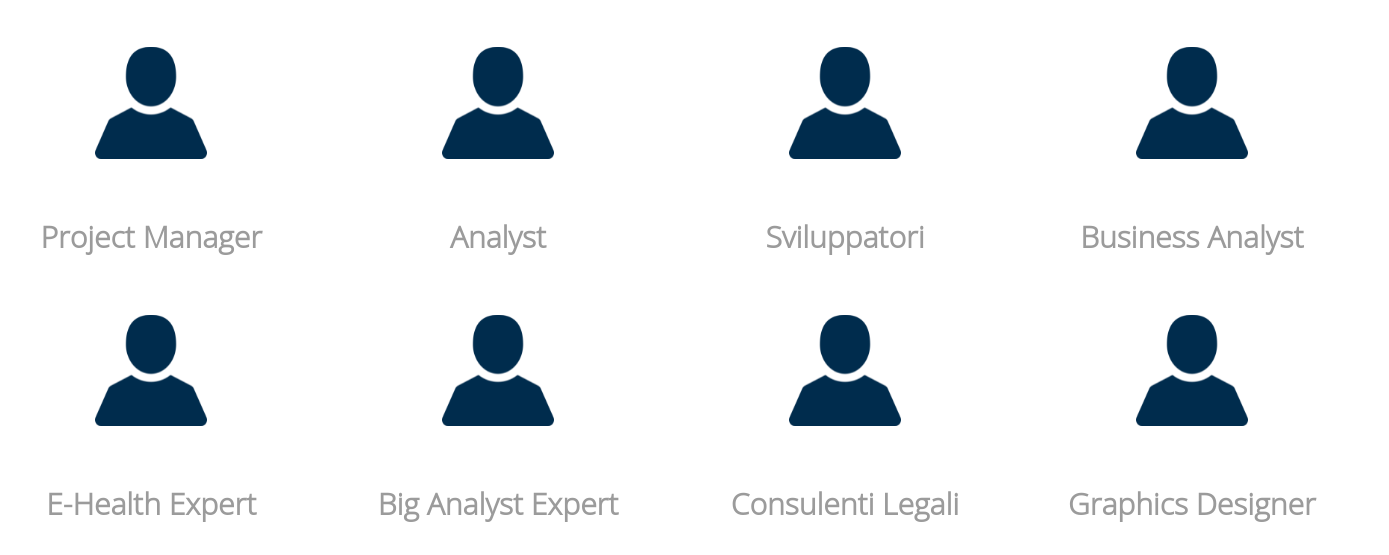
\includegraphics[width=\textwidth]{capitolo1/profili-professionali.png}
  \caption{I profili professionali messi a disposizione da Sync Lab}
  \textbf{Fonte}: \href{https://www.synclab.it/servizi-professionali.php}{https://www.synclab.it/servizi-professionali.php}
\end{figure}

In quanto \emph{partner} di grandi imprese italiane, come elencato nella sezione precedente, uno degli obiettivi principali di Sync Lab è quello di fornire una consulenza ai suoi clienti che porti un'evoluzione in termini di competitività, sviluppo e innovazione tecnologica. Inoltre, mette a disposizione un team di grande esperienza che interviene nella progettazione e realizzazione delle strategie necessari alla realizzazione di grandi progetti.

\subsection{Fornitura}
La procedura di fornitura viene avviata ogni qual volta che un cliente incarica Sync Lab per la realizzazione di un prodotto. Parallelamente, mette in atto le seguenti attività con lo scopo di migliorare questo processo:
\begin{itemize}
  \item \textbf{Miglioramento delle performance}: verifica e correzione, se necessario, delle procedure aziendali utilizzando le giuste metodologie (\emph{best practices});
  \item \textbf{Ottimizzazione della qualità}: utilizzo di \emph{design patterns} adatti al contesto aziendale;
  \item \textbf{Sviluppo delle quote di mercato}: analisi e miglioramento degli standard di qualità presso l'azienda.
\end{itemize} 

\subsection{Sviluppo}
Sync Lab fa ampio uso del modello di sviluppo Agile, più in particolare della metodologia Scrum, per permettere agli \emph{stakeholders} di seguire l'evoluzione dello sviluppo del prodotto richiesto, raccogliendo tutti i \emph{feedback} che possono essere determinanti per la loro soddisfazione. 

\paragraph{La metodologia Scrum}
Scrum è la metodologia Agile più diffusa tra i team di sviluppo. In questa metodologia gli \emph{stakeholders} hanno un ruolo fondamentale e la loro soddisfazione è determinante per la buona riuscita del progetto. Per rispondere al meglio a questa esigenza, si basa su tre pilastri fondamentali:
\begin{enumerate}
  \item \textbf{Trasparenza}: tutti coloro che partecipano ad un progetto sanno qual è lo scopo (trasparenza verticale) e sanno che cosa fanno gli altri (trasparenza orizzontale). In più, anche lo stato del progetto, con le relative statistiche, è visibile a tutti a prescindere dal livello organizzativo;
  \item \textbf{Ispezione}: ogni iterazione ed incremento vengono verificati in base alle metriche di misurazione decise, in modo tale da modificare le iterazioni successive e rendere così estremamente adattabile l'andamento del processo;
  \item \textbf{Adattamento}: è la conseguenza dell'ispezione e significa che al posto di seguire un piano preordinato, il team di sviluppo pianifica in base ai risultati dell'ispezione per apportare il maggior valore al cliente finale.
\end{enumerate}

\clearpage

\begin{figure}[h!]
  \centering
  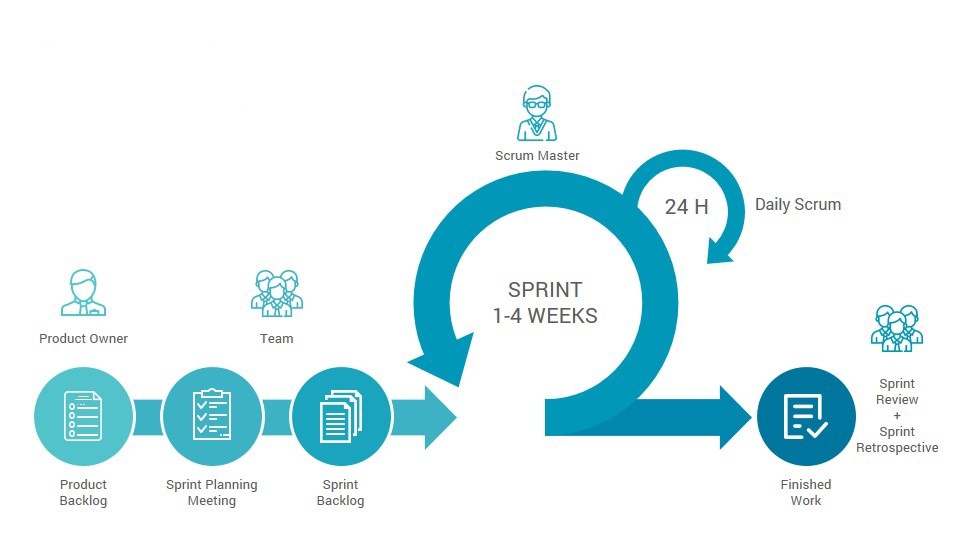
\includegraphics[width=0.8\textwidth]{capitolo1/scrum.jpeg}
  \caption{La metodologia Scrum}
\end{figure}

Durante il periodo di stage ho potuto osservare come vengono organizzati e gestiti i vari \emph{sprint} in Sync Lab. Ad ogni \emph{sprint} corrisponde l'introduzione di una nuova funzionalità che viene opportunamente verificata e comprovata dalla soddisfazione del cliente. L'esecuzione di uno \emph{sprint} prevederà i seguenti passi:
\begin{enumerate}
  \item si definisce un \textbf{\emph{product backlog}}, dove verranno riportate le attività da fare in una \emph{scrum board}, relative al progetto;
  \item si realizza uno \textbf{\emph{sprint planning}}, un sottoinsieme di obiettivi da raggiungere durante un singolo \emph{sprint} sulla base del \emph{product backlog};
  \item si esegue lo \textbf{\emph{sprint}} in un lasso di tempo limitato di massimo 4 settimane;
  \item si revisiona lo \textbf{\emph{sprint goal}} in cui si valuta l'incremento effettivo al termine dello \emph{sprint}.
\end{enumerate}

% \clearpage

\begin{figure}[h!]
  \centering
  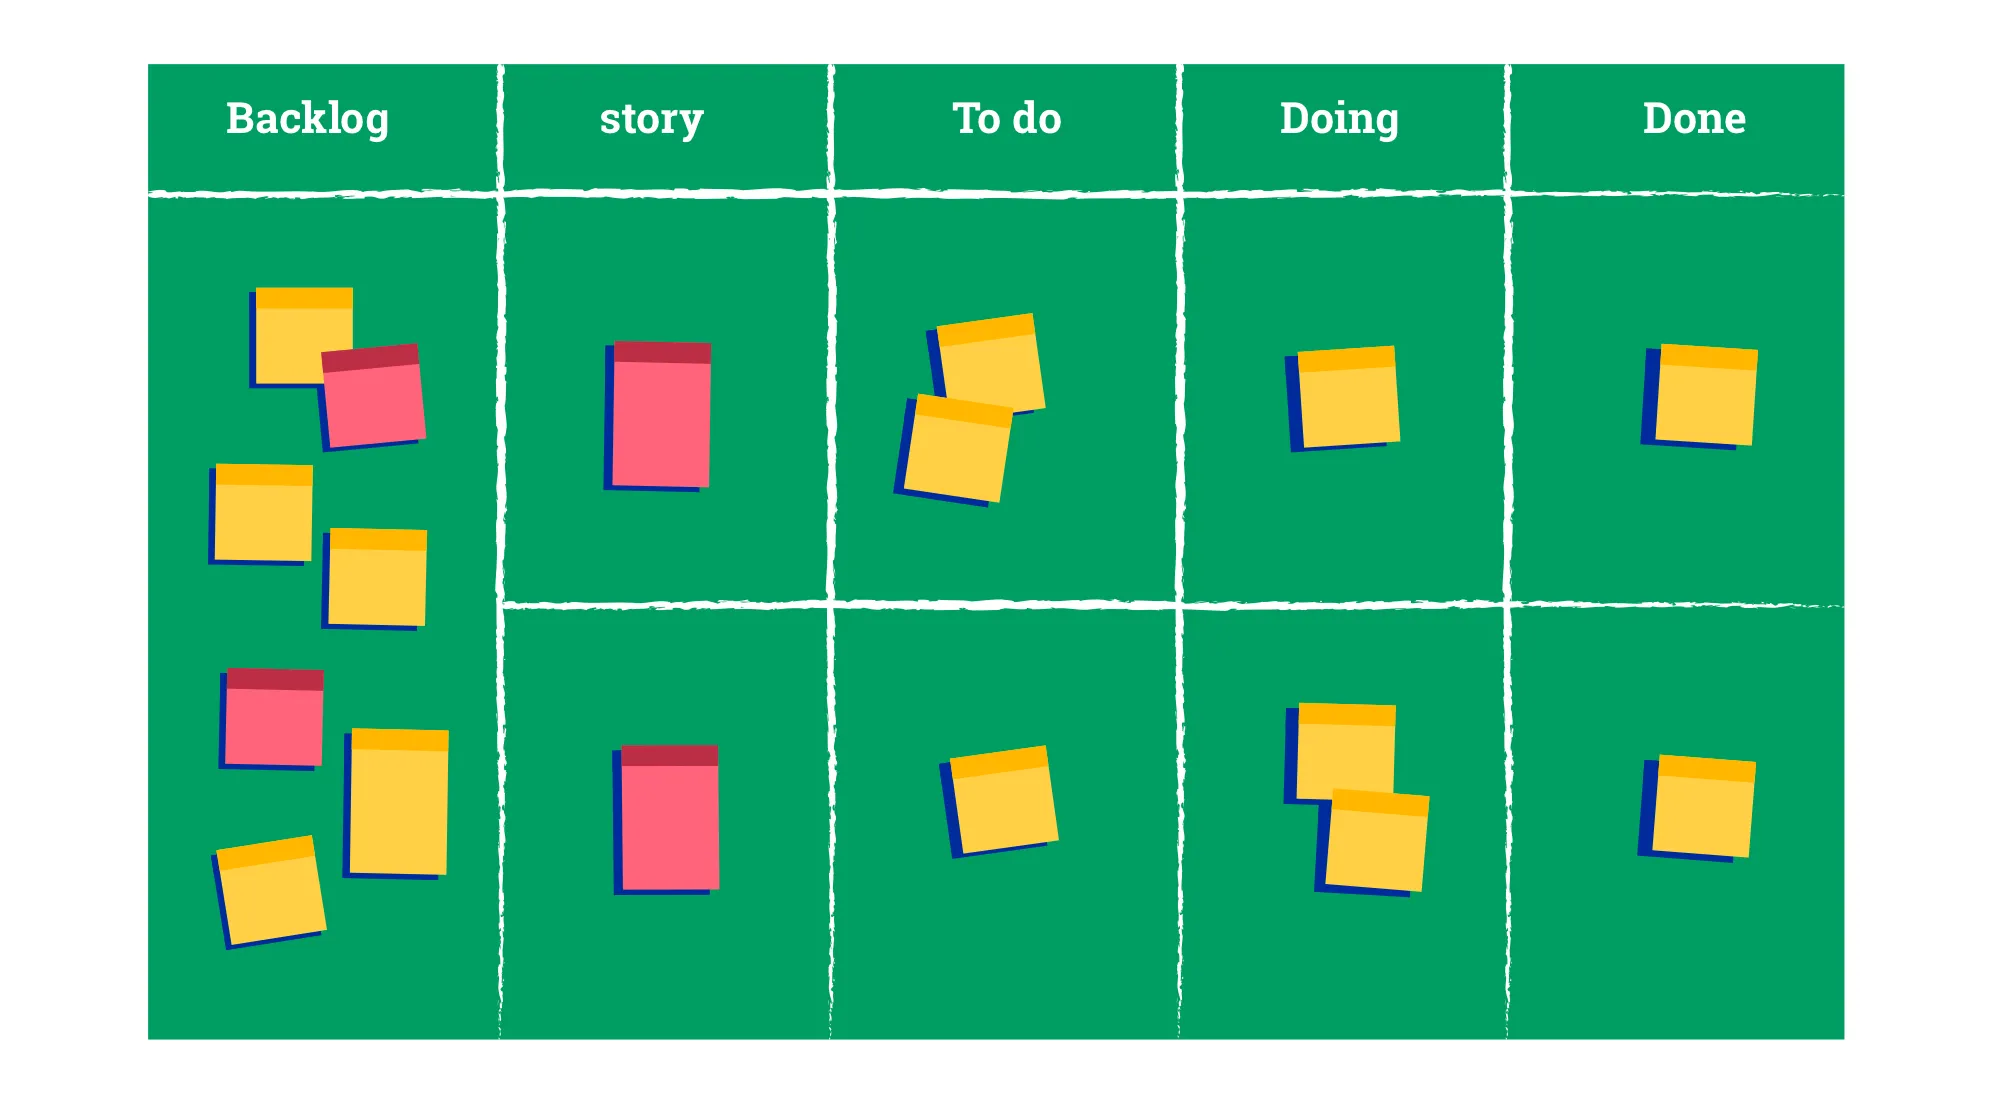
\includegraphics[width=0.8\columnwidth]{capitolo1/scrumb-board.png}
  \caption{Esempio di organizzazione delle attività nella Scrum Board}
\end{figure}

Un altro evento fondamentale che fa parte di Scrum, al quale ho avuto modo di partecipare, è lo \textbf{\emph{sprint review}}. Quest'ultimo consiste in una riunione di fine sprint in cui si ispezionano i risultati dell'incremento insieme agli \emph{stakeholders}, decidendo eventuali cambiamenti da apportare al \emph{product backlog}. \\

\subsection{Manutenzione}
In seguito al rilascio di un \emph{software}, l'azienda si impegna a seguire la sua naturale evoluzione nel tempo, adattandolo sempre a nuove esigenze, e a risolvere eventuali errori. Per questo Sync Lab offre servizi di manutenzione che possono essere di tre tipi:
\begin{itemize}
  \item \textbf{Manutenzione correttiva}: permette di correggere eventuali difetti del prodotto;
  \item \textbf{Manutenzione adattiva}: permette di adattare il \emph{software} a cambiamenti dell'ambiente operativo;
  \item \textbf{Manutenzione evolutiva}: permette di estendere le funzionalità del prodotto esistente.
\end{itemize}

\section{Tecnologie utilizzate}
Da quel che ho potuto constatare durante l'attività di stage, per la realizzazione dei prodotti sopra elencati Sync Lab sfrutta un'ampia gamma di tecnologie per fornire prodotti stabili e sicuri. Le tecnologie utilizzate sono molte e variano in base alla necessità del prodotto, ma quelle più utilizzate possono essere raggruppate in due grandi categorie: \emph{front-end} e \emph{back-end}. \\

Per quanto riguarda le tecnologie di supporto, c'è stato un aumento di utilizzo dei sistemi di comunicazione digitali a causa della pandemia, anche se venivano già utilizzati precedentemente per comunicare con le diverse sedi. La pandemia ha spinto Sync Lab ad un utilizzo sempre maggiore di Discord, Google Meet, Trello e Notion.

\begin{itemize}
  \item \textbf{Google Meet}: \emph{software} utilizzato per le videoconferenze che permette di comunicare con più colleghi aziendali e organizzare riunioni virtuali con un grande numero di partecipanti;
  \item \textbf{Discord}: piattaforma di comunicazione digitale gratuita, la quale permette di fruire di chat in tempo reale, gestendo più canali vocali e testuali divisi per argomento. Tra le varie funzioni disponibili, permette di dividere i membri in gruppi in base al progetto che devono portare a termine. È presente anche una sezione per le videoconferenze, ma è meno avanzata rispetto a Google Meet e per questo non lo si preferisce;
  \item \textbf{Trello}: piattaforma per la gestione di progetti seguendo la metodologia Scrum. Trello mette a disposizione una \emph{Scrum Board} dove è possibile dividere le attività in base al loro stato di avanzamento. Le colonne sono modificabili, come qualsiasi componente in Trello, ma quelle predefinite sono le seguenti:
  \begin{itemize}
    \item \textbf{Backlog}: contiene il \emph{product backlog};
    \item \textbf{Da fare}: definisce le attività da svolgere durante lo \emph{sprint};
    \item \textbf{In corso}: presenta tutte le attività in esecuzione;
    \item \textbf{In verifica}: consiste in tutte le attività in attesa di verifica;
    \item \textbf{Terminati}: include le attività legate ad uno \emph{sprint} che sono state verificate. 
  \end{itemize}
  \item \textbf{Notion}: piattaforma utilizzata per la prenotazione del posto in sede, così da facilitare la gestione ed il controllo delle persone, in modo tale da rispettare il numero massimo consentito dalla legge.
\end{itemize}

\subsection{Front-end}
Le tecnologie per lo sviluppo di interfacce grafiche utilizzate da Sync Lab sono le seguenti:

\paragraph{Linguaggi di programmazione} 
I linguaggi di programmazione più utilizzati sono \textbf{Javascript}, impiegato nella realizzazione di applicativi web interattivi, \textbf{kotlin}, un linguaggio multi-paradigma che sta sempre più prendendo piede per lo sviluppo di applicazioni android, e \textbf{Swift}, per lo sviluppo di applicazioni IOS. Sempre di più si sta puntando su \textbf{Typescript}, un \emph{superset} di Javascript, al quale aggiunge tipi, classi e interfacce.

\paragraph{Framework}
L'ambito web è quello dove avviene un impiego maggiore di \emph{framework}. I più utilizzati sono attualmente due: Angular e React.js. \textbf{Angular} è uno dei \emph{framework} open-source più popolari e utilizzati al mondo per lo sviluppo di \gls{Single Page Application}. Permette di creare applicazioni web di livello \emph{enterprise} grazie a una serie di funzionalità e strumenti, utilizzando come linguaggio principale Typescript. \textbf{React.js}, invece, si distingue da Angular per la maggiore facilità di apprendimento e velocità a livello di \emph{performance}, la quale lo rende perfetto per la realizzazione di siti semplici. Un altro \emph{framework} che sta sempre di più prendendo piede all'interno dell'azienda, anche se di fatto non è ancora stato adottato ufficialmente, è \textbf{Vue.js}. Molto simile a React.js, Vue.js introduce il concetto di \gls{Single File Components}, semplificando maggiormente la scrittura di applicazioni web.

\subsection{Back-end}
Per quanto riguarda le tecnologie per lo sviluppo lato \emph{back-end}, si possono identificare le seguenti:

\paragraph{Linguaggi di programmazione}
\textbf{Java} e \textbf{Scala}, due linguaggi basati sulla \emph{Java Virtual Machine}, fanno da padrone per lo sviluppo lato \emph{back-end}. Entrambi sono linguaggi maturi ed ampiamente utilizzati in questo mondo, con una grande varietà di librerie e \emph{framework}. Vengono sfruttati principalmente per lo sviluppo di servizi \emph{REST} in ambito web.

\paragraph{Framework}
Il \emph{framework} più utilizzato per lo sviluppo in questo ambito è sicuramente \textbf{Spring}. Quest'ultimo permette di realizzare applicativi lato \emph{server} utilizzando il linguaggio Java e sfruttando vari \emph{design patterns}. La scelta dell'architettura è totalmente libera e Spring si presta perfettamente a qualunque tipologia si voglia scegliere.

\section{Propensione all'innovazione}
Sync Lab è un'azienda in costante aggiornamento che guarda all'innovazione con grande interesse, per garantire soluzioni software sempre rivoluzionarie. Simbolo di questo sforzo da parte dell'azienda è anche la grande quantità di collaborazioni con le principali università d'Italia (università degli studi di Padova, politecnico di Milano, università degli studi Federico II, ecc.) e vari enti europei.\\

\begin{figure}[!h]
  \centering
  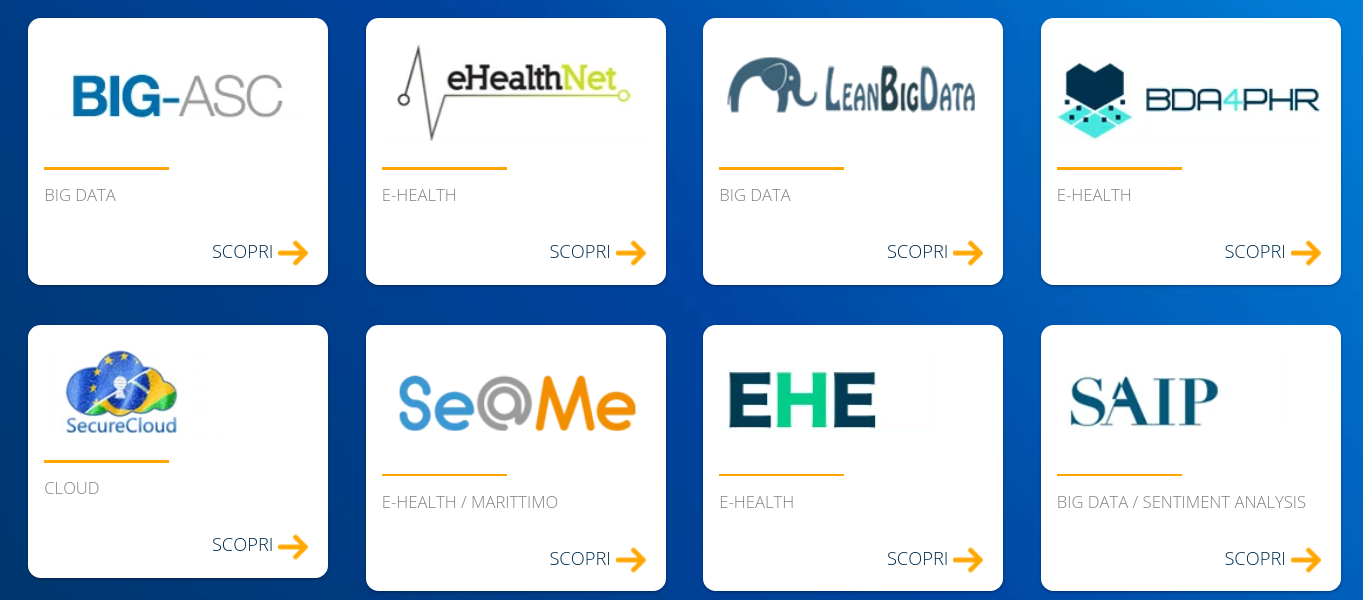
\includegraphics[width=\textwidth]{capitolo1/prodotti-ricerca-sviluppo.png}
  \caption{Alcuni progetti di ricerca e sviluppo di Sync Lab}
  \textbf{Fonte}: \href{https://www.synclab.it/ricerca-e-sviluppo.php}{https://www.synclab.it/ricerca-e-sviluppo.php}
\end{figure}

Per adempiere al meglio al difficile compito di restare sempre aggiornati sulle ultime tecnologie, Sync Lab è divisa in tre dipartimenti:
\begin{itemize}
  \item \textbf{\emph{Research and Development (R\&D)}}: dove l'azienda promuove nuovi prodotti eseguendo ricerca e sviluppo in più settori, alimentando così il profilo aziendale e le proprie competenze nel mercato;
  \item \textbf{\emph{Lab}}: in cui l'azienda mette in atto i risultati derivanti dal dipartimento \emph{R\&D}, promuovendo soluzioni che migliorino ed estendano l'innovazione tecnologica;
  \item \textbf{\emph{Start-up}}: dove l'azienda collabora e promuove le \emph{start-up} con maggiore successo in termini di innovazione, sia in Italia che all'estero.
\end{itemize}  

L'azienda, inoltre, sta approfondendo sempre di più gli ambiti di \emph{Cybersecurity}, \emph{E-Health}, \emph{Blockchain} e \emph{Big Data}, formando degli appositi progetti di ricerca nelle diverse sedi per sperimentare e imparare nuove tecnologie. \\

Un evento che ho trovato interessante e mi è piaciuto molto durante il mio tirocinio, è stato il "Paola presenta". 
Questa ricorrenza, che in genere è settimanale, consiste in un'ora di presentazione su un argomento proposto da un dipendente. L'argomento della presentazione può riguardare qualcosa sulla quale sta lavorando, oppure semplicemente si è interessato. 
Ogni dipendente è libero di partecipare e, su richiesta, può presentare lui stesso un argomento a piacere. Questo evento l'ho trovato molto interessante e dimostra quanto i colleghi di Sync Lab vogliano sempre stare aggiornati ed informati su tutto quello che interessa il mondo informatico. 
Personalmente ho partecipato a tre di queste presentazioni: una dove hanno introdotto la tecnologia \emph{Blockchain}, tenuta dal mio \emph{tutor} aziendale Fabio Pallaro, un'altra dove hanno spiegato come funzionano gli strumenti che compongono la \emph{Elastick Stack} e l'ultima dove hanno parlato dell'analisi statica del codice con la piattaforma \emph{SonarQube}. \\

Questa propensione all'innovazione l'ho avvertita anche nel mio progetto di stage, dove non ho trattato tecnologie usuali, ma ho dovuto studiare e approfondire tecnologie che attualmente non sono così diffuse in ambito \emph{enterprise}, ma sicuramente rappresentano un'importante \emph{milestone} nella storia dell'informatica.
